%\documentclass[sigconf,review,anonymous]{acmart}
\documentclass[sigconf]{acmart}

\usepackage{amsfonts}
\usepackage[latin1]{inputenc}
\usepackage[english]{babel}
\usepackage{listings}
\usepackage{algorithmic}
\usepackage{float}
%\usepackage[numbers,sort&compress,square]{natbib}
\usepackage{graphicx}
\usepackage{booktabs}
\usepackage{subcaption}
%\usepackage{hyperref}
\usepackage{color}
%\usepackage[usenames,dvipsnames,table]{xcolor}
\usepackage{soul}
\usepackage{xspace}
\usepackage{boxedminipage}
\usepackage{alltt}
\usepackage{multirow}
\usepackage{paralist}
\usepackage{amsmath}
\usepackage{balance}
\definecolor{light-gray}{gray}{0.90}

\floatstyle{ruled}
\newfloat{algorithm}{tbp}{loa}
\floatname{algorithm}{Algorithm}

\newtheorem{definition}{Definition}


 %krams hinter fontadjust ist neu
  \definecolor{lightgrey}{rgb}{0.90,0.90,0.90}
\lstset{escapeinside={(*}{*)}}
  \lstloadlanguages{java}
 \lstdefinelanguage{pseudocode}
  {morekeywords={if, else, initialize, return, for, each, in, global, new}
   }
  \lstset{
    tabsize=2,
    mathescape=true,
    escapeinside={(*}{*)},
    captionpos=t,
    framerule=0pt,
    backgroundcolor=\color{lightgrey},
    basicstyle=\scriptsize\ttfamily,
    keywordstyle=\footnotesize\bfseries,
    numbers=none,
    numberstyle=\tiny,
    numbersep=1pt,
    fontadjust,
    breaklines=true,
    breakatwhitespace=false
  }


% \hypersetup{
% colorlinks=true,
% urlcolor=rltblue,
% linkcolor=rltred,
% citecolor=rltgreen,
% bookmarksnumbered=true,
% pdftitle={EvoSuite at the SBST 2016 Tool Competition},
% pdfauthor={Gordon Fraser and Andrea Arcuri},
% pdfsubject={Test case generation},
% pdfkeywords={Test case generation, unit testing, test
%   oracles, assertions, search based testing}
% }

\definecolor{rltred}{rgb}{0.5,0,0}
\definecolor{rltgreen}{rgb}{0,0.5,0}
\definecolor{rltblue}{rgb}{0,0,0.5}
\definecolor{ScarletRed}{rgb}{0.80,0.00,0.00}



% in draft mode we put \remarks into the margins and do other stuff
% set to \draftfalse for
\newif\ifdraft
\draftfalse

\ifdraft
	\marginparwidth=1.3cm
	\marginparsep=5pt
	\newcommand\remark[1]{%
		\mymarginpar{\raggedright\hbadness=10000\tiny\it #1\par}}
	% TODO marker
	\newcommand{\TODO}[1]{\sethlcolor{yellow}\textbf{\textcolor{ScarletRed}{\hl{TODO: #1}}}\xspace}
\else
	\newcommand\remark[1]	{}
	\newcommand{\TODO}[1]{}
\fi

\ifdraft
	\overfullrule3pt
\fi

% We use \FIXME for located problems (``defect'')
\newcommand{\FIXME}[1]{\remark{FIXME: #1}}
\newcommand\parremark[1]	{\par\textbf{REMARK:} #1\par}

\newcommand{\gordon}[1]{\textcolor{blue}{\sf\small\textbf{Gordon:} #1}}
\newcommand{\andrea}[1]{\textcolor{ScarletRed}{\sf\small\textbf{Andrea:} #1}}

% \mathid is used to denote identifiers and slots in formulas
\newcommand{\mathid}[1]{\text{\rmfamily\textit{#1}}}

% But usually, we shall use \|name| instead.
\def\|#1|{\mathid{#1}}

% \codeid is used to denote computer code identifiers
\newcommand{\codeid}[1]{\texttt{#1}}

% But usually, we shall use \<name> instead.
\def\<#1>{\codeid{#1}}

% Our results
\newenvironment{result}%
{\smallskip
\noindent
\let\emph=\textbf
\begin{boxedminipage}{\columnwidth}\begin{center}\em}%
{\end{center}\end{boxedminipage}%
\smallskip
}

\newcommand{\project}[1]{\textsc{#1}\xspace}
\newcommand{\Collections}{\project{Collections}}
\newcommand{\Threeten}{\project{Threeten}}
\newcommand{\Spatial}{\project{Spatial4j}}

\newcommand{\EVOSUITE}{\textsc{EvoSuite}\xspace}
\newcommand{\JTEXPERT}{\textsc{jTExpert}\xspace}
\newcommand{\RANDOOP}{\textsc{Randoop}\xspace}
\newcommand{\TT}{\textsc{T3}\xspace}

\newcommand{\MUTEST}{{\sc $\mu$Test}\xspace}
\newcommand{\CS}{{\sc SF100}\xspace}


\DeclareMathSymbol{,}{\mathpunct}{letters}{"3B}
\DeclareMathSymbol{,}{\mathord}{letters}{"3B}
\DeclareMathSymbol{\decimal}{\mathord}{letters}{"3A}
%%%"

\usepackage{siunitx}
\newcommand{\score}{\num{380.57}\xspace}
\newcommand{\cuts}{\num{65}\xspace}
\newcommand{\budgetShort}{\SI{30}{\second}\xspace}
\newcommand{\budgetLong}{\SI{120}{\second}\xspace}
\newcommand{\avgLinesCoverageRatioShort}{\SI[round-mode=figures,round-precision=3]{51.87307894984616}{\percent}\xspace}
\newcommand{\medLinesCoverageRatioShort}{\SI[round-mode=figures,round-precision=3]{46.666668}{\percent}\xspace}
\newcommand{\avgLinesCoverageRatioLong}{\SI[round-mode=figures,round-precision=3]{62.73892781107692}{\percent}\xspace}
\newcommand{\medLinesCoverageRatioLong}{\SI[round-mode=figures,round-precision=3]{71.71428499999999}{\percent}\xspace}
\newcommand{\avgConditionsCoverageRatioShort}{\SI[round-mode=figures,round-precision=3]{46.11903214169231}{\percent}\xspace}
\newcommand{\medConditionsCoverageRatioShort}{\SI[round-mode=figures,round-precision=3]{47.22222}{\percent}\xspace}
\newcommand{\avgConditionsCoverageRatioLong}{\SI[round-mode=figures,round-precision=3]{56.821364993692306}{\percent}\xspace}
\newcommand{\medConditionsCoverageRatioLong}{\SI[round-mode=figures,round-precision=3]{60.000004}{\percent}\xspace}
\newcommand{\avgMutantsCoverageRatioShort}{\SI[round-mode=figures,round-precision=3]{39.44754914507693}{\percent}\xspace}
\newcommand{\medMutantsCoverageRatioShort}{\SI[round-mode=figures,round-precision=3]{20.353981}{\percent}\xspace}
\newcommand{\avgMutantsCoverageRatioLong}{\SI[round-mode=figures,round-precision=3]{34.111612112}{\percent}\xspace}
\newcommand{\medMutantsCoverageRatioLong}{\SI[round-mode=figures,round-precision=3]{0.0}{\percent}\xspace}
\newcommand{\numTestGenFailedShort}{\num{21}\xspace}
\newcommand{\numTestGenFailedLong}{\num{26}\xspace}


\copyrightyear{2022}
\acmYear{2022}
\setcopyright{acmcopyright}
\acmConference[SBST'22 ]{The 15th Search-Based Software Testing Workshop}{May 9, 2022}{Pittsburgh, PA, USA}
\acmBooktitle{The 15th Search-Based Software Testing Workshop (SBST'22 ), May 9, 2022, Pittsburgh, PA, USA}
\acmPrice{15.00}
\acmDOI{10.1145/3526072.3527526}
\acmISBN{978-1-4503-9318-8/22/05}

%-------------------------------------------------------------------------
% take the % away on next line to produce the final camera-ready version
\pagestyle{empty}

%-------------------------------------------------------------------------
\begin{document}

%

%\title{Unit Testing Tool competition: Results for EvoSuite}
\title{\EVOSUITE at the SBFT 2023 Tool Competition}


\author{Sebastian Schweikl}
\affiliation{%
  \institution{University of Passau}
  \city{Passau}
  \country{Germany}
}
%\email{gordon.fraser@uni-passau.de}

\author{Gordon Fraser}
\affiliation{%
  \institution{University of Passau}
  \city{Passau}
  \country{Germany}
}
%\email{gordon.fraser@uni-passau.de}

\author{Andrea Arcuri}
\affiliation{%
  \institution{Kristiania University College and Oslo Metropolitan University}
  \city{Oslo}
  \country{Norway}
}
%\thispagestyle{empty}

\begin{abstract}
  \EVOSUITE is a search-based unit test generation tool for Java. This paper summarises the results and experiences of \EVOSUITE's participation at the 11th unit testing competition at SBFT 2023, where \EVOSUITE achieved the highest overall score.
\end{abstract}

\maketitle

%-------------------------------------------------------------------------
\section{Introduction}
%
For the last 10 years, the annual unit test generation competition has
evaluated progress on unit test generation tools using a benchmark of Java
classes, on which different tools are applied and compared. In the 2023 edition
of the competition, five tools were applied on a set of \cuts classes. Details
about the procedure of the competition, the technical framework, and the
benchmark classes can be found in the competition
report~\cite{SBST-toolcomp22}. \EVOSUITE achieved an overall score of \score,
which was the highest among the competing and baseline tools.


%-------------------------------------------------------------------------
\section{About EvoSuite}


\EVOSUITE~\cite{FrA11c} automatically generates test suites for Java classes
using evolutionary search. As input \EVOSUITE only requires the name of the
target class as well as the classpath on which the compiled bytecode of the
target class and its dependencies are located. \EVOSUITE first extracts
information about the relevant classes as well as their constructors, methods,
and fields using a basic static analysis. It instruments the bytecode while
classes are loaded by the Java classloader, such that \EVOSUITE can produce
execution traces for test executions, and to avoid test flakiness by replacing
non-deterministic calls with deterministic, mocked versions. Finally, \EVOSUITE
applies meta-heuristic search algorithms to automatically produce JUnit test
cases aimed at maximising code coverage.
%Besides the basic command line interface there are also plugins for popular development environments such as IntelliJ, Eclipse, or Maven~\cite{ICST16_Tool}.


\EVOSUITE generates tests using evolutionary algorithms.
%
For this, it uses a genetic encoding of test cases consisting of variable-length sequences of Java statements (e.g., primitive statements as well as calls on constructors or methods). Standard evolutionary search operators (e.g., selection, crossover, mutation) are adapted for this representation.
%
\EVOSUITE provides several different evolutionary algorithms to operate on this
representation. The initial approach was to optimise entire test suites with
respect to their overall code coverage~\cite{GoA_TSE12}. However, after
extensive evaluation~\cite{ea_evaluation} the default is now the
\emph{Dynamic Many-Objective Sorting Algorithm} (DynaMOSA) search
algorithm~\cite{dynamosa}, which operates at the test case level.
%
The search is driven by fitness functions that encode coverage criteria. \EVOSUITE can optimise for several criteria simultaneously, and the core fitness functions in \EVOSUITE are based on traditional heuristics for code coverage, such as the branch distance and the approach level (see~\cite{GoA_TSE12} for more details). However, there are several further fitness functions based on mutation testing~\cite{emse14_mutation} as well as other basic criteria~\cite{rojas2015combining}.


A large share of the complexity of \EVOSUITE's code base is due to efforts to
avoid flakiness in the generated tests. On the one hand, this covers extensive
instrumentation and mocking. On the other hand, \EVOSUITE also compiles and
executes each test individually to avoid compilation errors (which may be the
result of bugs in \EVOSUITE) or flakiness caused by non-determinism in the
class under test.

\EVOSUITE is also heavily optimised in order to produce tests that are as readable as possible and avoid test smells~\cite{panichella2020revisiting}. For this, \EVOSUITE applies post-processing once the available search budget has been exhausted~\cite{FrA11c,FrA13a}, consisting of minimisation to remove redundant tests and statements, and adding a minimised set of assertions using mutation analysis~\cite{10.1109/TSE.2011.93}.
%Besides multiple in-depth empirical evaluations of \EVOSUITE with respect to
%code coverage~\cite{fraser2014large,emse_archive,ea_evaluation,dynamosa},
%fault-finding effectiveness~\cite{shamshiri2015automatically,moein2017}, and
%effects on developer productivity~\cite{TOSEM_userstudy,ISSTA15_Study} and
%software maintenance~\cite{ICST2018_Maintenance}, \EVOSUITE has also participated in all prior instances of the unit testing tool competition, usually ranking among the best performing tools.





%-------------------------------------------------------------------------
\section{Competition Setup}

The 2023 competition setup was similar to the 2022 setup: The same version of
\EVOSUITE (1.1.0) was used, which by default uses DynaMOSA~\cite{dynamosa} as
the search algorithm.
% No new features were added in this version, but support
% for Java 9+ was added, several bugs were fixed, and amajor refactoring was applied
% to improve the code quality with respect to the
% use of Java Generics internally. While several smaller bugfixes were applied in
% the run-up to the 2021 competition, no further optimisation or testing was
% applied for 2022.

The configuration is largely identical to the established configuration used in
prior years, and mainly uses the tuned default
values~\cite{arcuri2013parameter} and default coverage criteria
\cite{rojas2015combining}.
%
Unlike previous years, where the competition score did not yet reward readability,
the configuration now enables a test minimisation step, and filters regression
assertions using mutation analysis.
%
The time budget was again distributed by allocating \SI{50}{\percent} of the overall time
set by the competition organisers for the search, and the other \SI{50}{\percent} equally to
the remaining phases (e.g., assertion generation, compile-check, flakiness-check).



%-------------------------------------------------------------------------
\section{Results}

%\begin{figure}
%  \centering
%  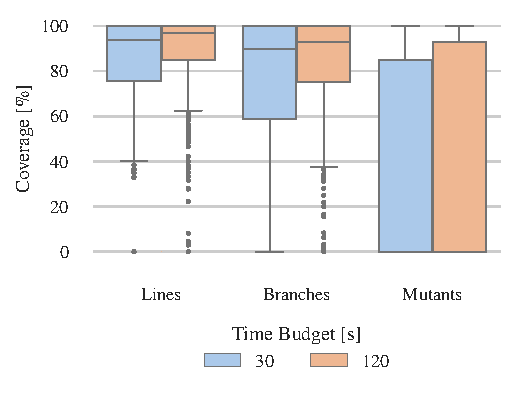
\includegraphics[width=\columnwidth]{data/CoverageBoxV}
%  \caption{Coverage results achieved in the competition.}
%  \label{fig:results}
%\end{figure}

\begin{figure}
  \centering

  \begin{subfigure}{0.9\columnwidth}
    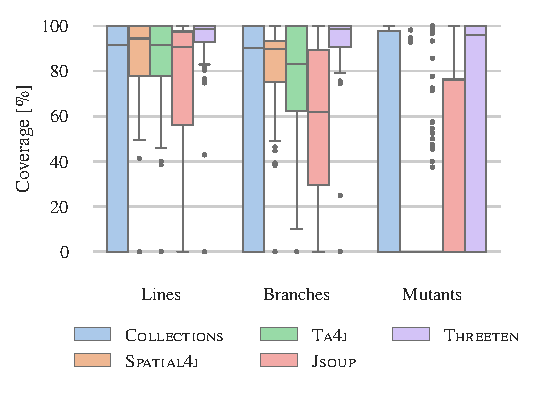
\includegraphics[width=\linewidth]{data/CoverageByBenchmark30.pdf}
    \caption{Coverage results achieved in the competition with \SI{30}{\second}.}
    \label{fig:results30}
  \end{subfigure}

  \begin{subfigure}{0.9\columnwidth}
    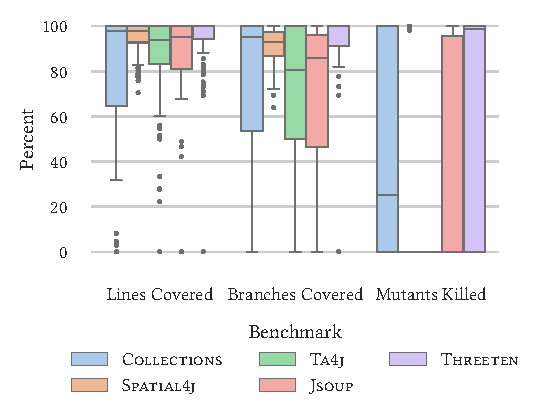
\includegraphics[width=\linewidth]{data/CoverageByBenchmark120.pdf}
    \caption{Coverage results achieved in the competition with \SI{120}{\second}.}
    \label{fig:results120}
  \end{subfigure}

  \caption{Competition results achieved by \EVOSUITE summarised by projects from which the classes under test.}
  \label{fig:figures}
\end{figure}


With an overall score of \score, \EVOSUITE achieved the highest score of all
tools in the competition. As described in the competition
report~\cite{SBST-toolcomp22}, the score is the weighted sum between the
rankings for coverage and understandability.

Figure~\ref{fig:results30} summarises the results of \EVOSUITE in terms of the
mean coverage for the \cuts classes used in the competition for the \budgetShort search budget; Figure~\ref{fig:results120} shows the results for the \budgetLong search budget. The coverage
increased from the \budgetShort to the \budgetLong search budget (mean line
coverage of \avgLinesCoverageRatioShort vs. \avgLinesCoverageRatioLong, respectively).

\EVOSUITE failed to generate any tests in \numTestGenFailedShort cases with a
budget of \budgetShort, and in \numTestGenFailedLong cases with a budget of
\budgetLong. However, we found no crashes of \EVOSUITE itself (e.g., exceptions
thrown by \EVOSUITE), but in all cases where no tests were generated the
\EVOSUITE process had been killed by the competition setup, suggesting that
\EVOSUITE was using more time than allocated.

While the results for line coverage and branch coverage are similar, the
mutation scores are substantially lower. The mutation scores on the \Threeten
classes are highest compared to the other projects from which classes were taken.

For the first time, the competition also conducted a human study with 13
participants to assess test case readability. To this, a method under test
was chosen for each of the \Collections, \Threeten, and \Spatial
projects. Then, for each competitor a test covering that method was selected
randomly among the generated ones. Finally, the participants were asked
to rank the tests for each project on a scale from 1 (best) to 5 (worst),
in terms of readability. Overall, \EVOSUITE achieved the 2nd highest rank
rating. Its distribution is shown in Figure~\ref{fig:readability}.

Most participants found \EVOSUITE-generated tests to be readable. When
\EVOSUITE ranked highest, they positively highlighted the thoroughness of
generated assertions, using edge cases as inputs, and the fact that tests
where short. When \EVOSUITE ranked lowest, participants criticised the lack
of comments and descriptive test names, repetitiveness in the code, and
needless assertions.

Among the tests for \Collections the longest one was produced by \EVOSUITE.
Interestingly, it ranked both highest and lowest, with one participant
stating it was ``the most complete'', while another suggested the code
being longer makes it ``more confusing''.


\begin{figure}
  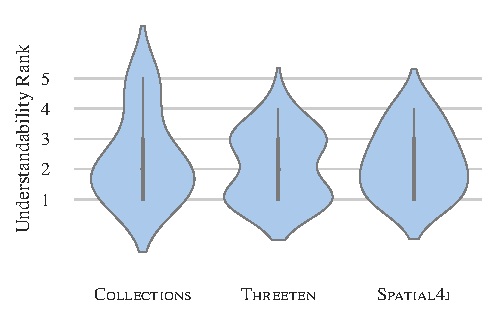
\includegraphics[width=0.9\columnwidth]{./data/understandability}
  \caption{Distribution of test case understandability, ranked from 1 (best) to 5 (worst), per project.}
  \label{fig:readability}
\end{figure}


%-------------------------------------------------------------------------
\section{Conclusions}

This paper reports on the participation of the \EVOSUITE test generation tool
in the tenth SBST Java Unit Testing Tool Contest. On average, \EVOSUITE
achieved \avgConditionsCoverageRatioLong branch coverage,
\avgLinesCoverageRatioLong line coverage, and a mutation score of
\avgMutantsCoverageRatioLong, using a search budget of \budgetLong on the \cuts
classes considered for the competition. Overall, this results in a score of
\score, which is the highest score of all tools in the competition.


To learn more about \EVOSUITE, visit our Web site:
\begin{center}
%\url{http://evosuite.org/}
\texttt{http://www.evosuite.org}
\end{center}


%-------------------------------------------------------------------------

%\noindent
\textbf{Acknowledgments:} Many thanks to all the contributors to
\EVOSUITE.
%This project has been supported by EPSRC project % ``GREATEST''
%EP/N023978/2.


%-------------------------------------------------------------------------
%\def\IEEEbibitemsep{5pt plus 1pt}
%\def\IEEEbibitemsep{6pt}
%\clearpage
\bibliographystyle{IEEEtranS}
\bibliography{papers}
\balance

\end{document}


%%% Local Variables:
%%% mode: latex
%%% TeX-master: t
%%% End:
